\section{Visualizing and Understanding}

\subsection{First Layer: Visualize Filters}

对于第一层卷积层，我们可以可视化每个卷积核的权重，并得到一系列可解释的图片：

\begin{figure}[H]
    \centering
    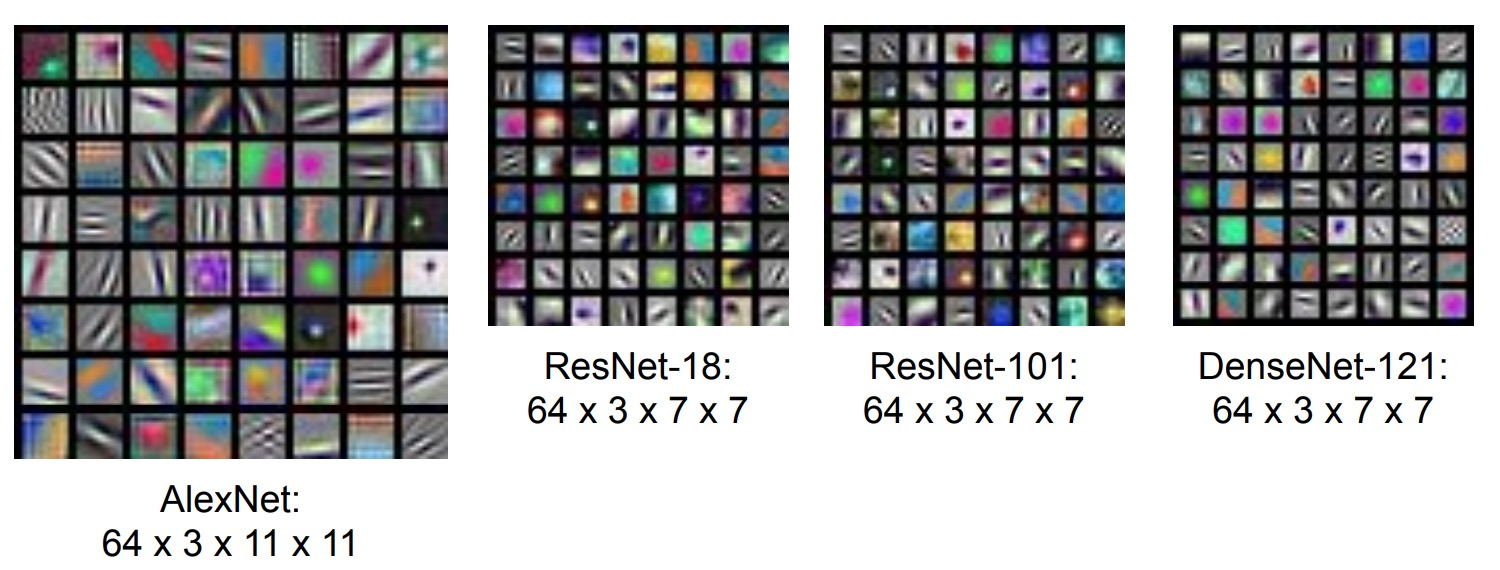
\includegraphics[width=0.8\linewidth]{figs/chapter7/first.jpg}
\end{figure}

可以看出，第一层卷积层在寻找一些点与线，以及对立的颜色，可以认为是在寻找物体与物体之间的分割线。

为什么可视化卷积核的权重是有道理的呢？卷积核所做的就是与所有训练数据进行内积运算，而我们知道，两个向量越相近，其内积结果越大，因此，卷积核图片上的一条白线，可以认为是众多数据中存在这么一条线，使得卷积核学到了这一特征。

\subsection{Last Layer}

\paragraph{Nearst Neighbors}

最后一层的输出其实可以看作是每个图像的特征向量，因此我们可以画出 nearst neighbors：

\begin{figure}[H]
    \centering
    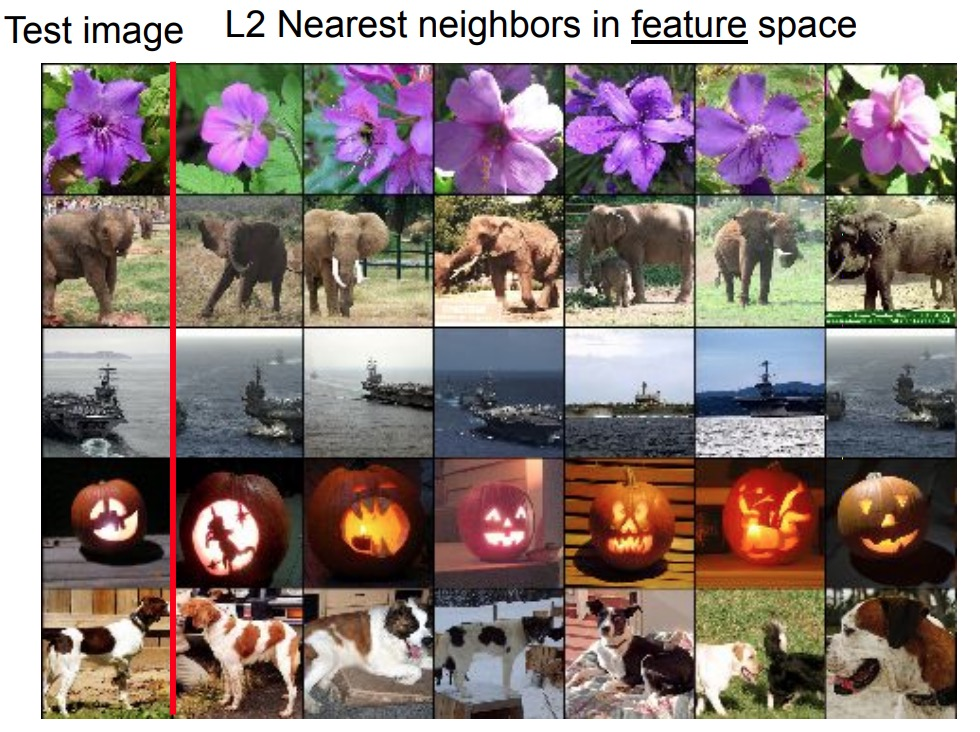
\includegraphics[width=0.8\linewidth]{figs/chapter7/last-nn.jpg}
\end{figure}

可以看见，这比我们在第一节课直接用像素空间进行距离的衡量要准确很多。

\paragraph{Dimensionality Reduction}

将最后一层的向量使用降维方法，例如简单的 PCA 或更强大的 \textbf{t-SNE} 降维至 $2$ 维并作图。

在 MNIST 上，我们可以得到：

\begin{figure}[H]
    \centering
    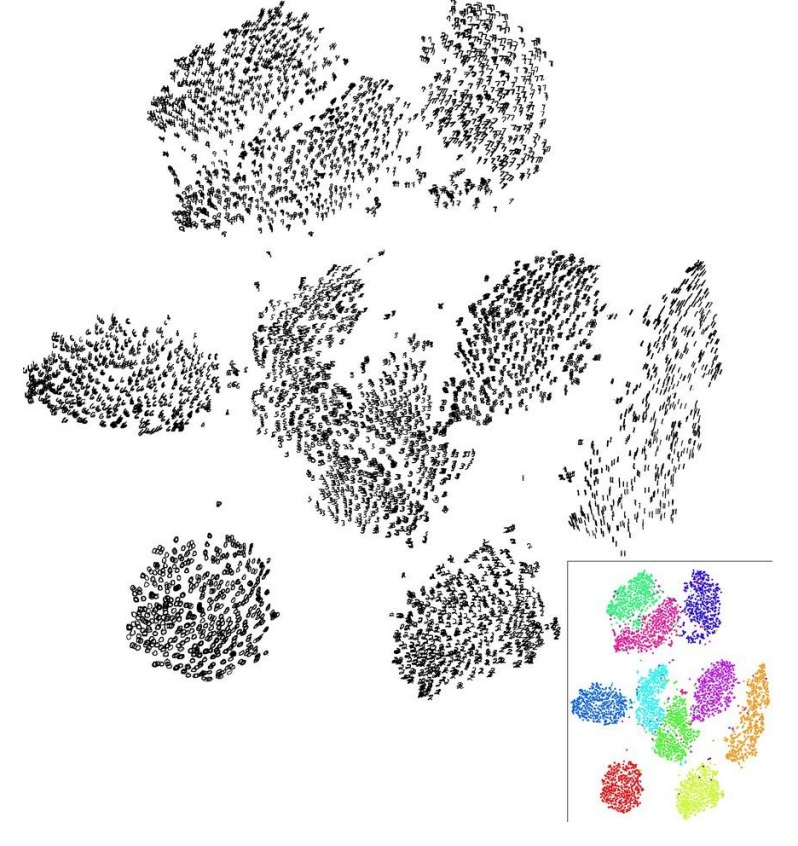
\includegraphics[width=0.5\linewidth]{figs/chapter7/last-dr.jpg}
\end{figure}

在 CIFAR-10 上，我们把降维后的点放置在网格中（准确来讲，是找出与每个网格点中心最相似的图片），得到如下可视化结果（高清版本参见 \url{http://cs.stanford.edu/people/karpathy/cnnembed/}）：

\begin{figure}[H]
    \centering
    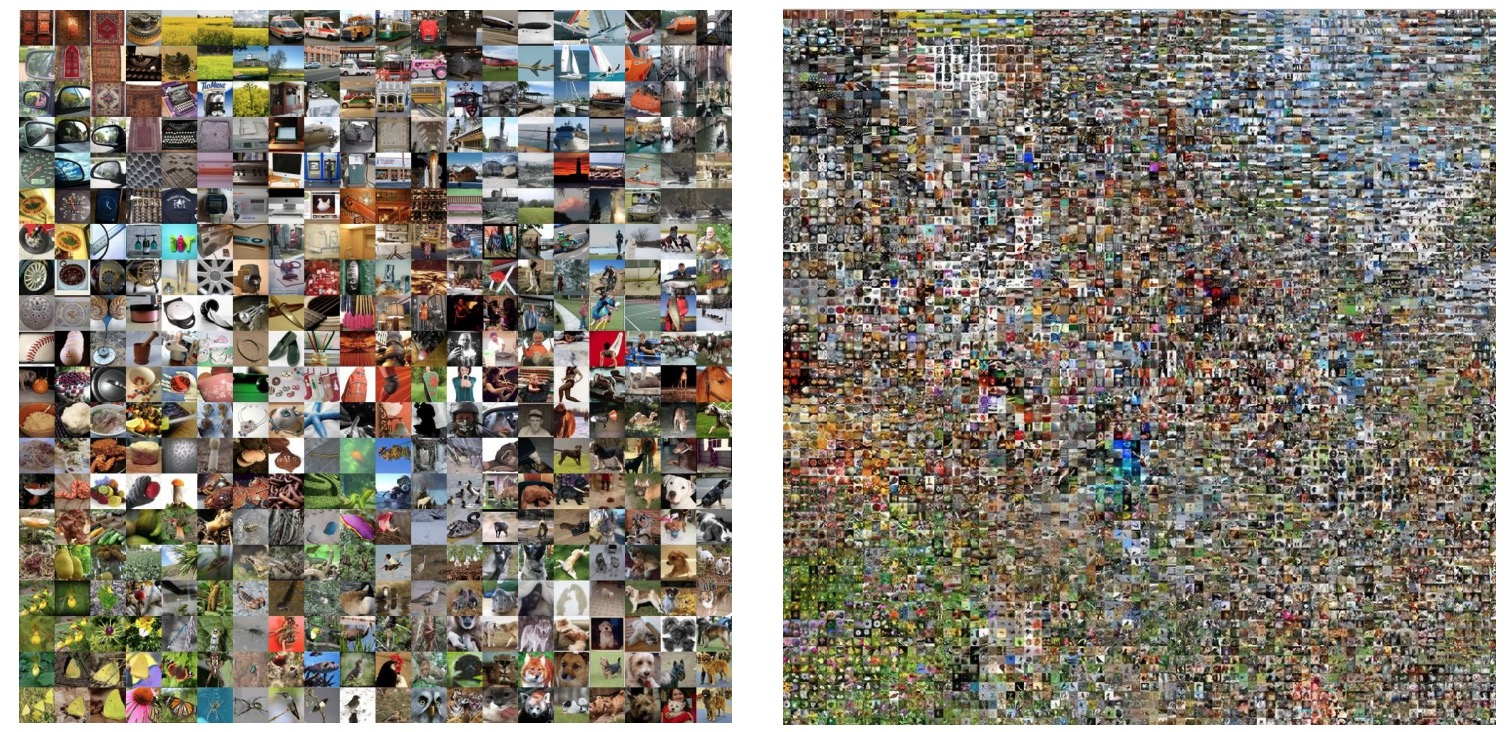
\includegraphics[width=0.8\linewidth]{figs/chapter7/last-dr2.jpg}
\end{figure}

\subsection{Maximally Activating Patches}

从网络中选择某层的某个 channel，输入若干图片并记录这个 channel 上的数值。由于使用的是卷积神经网络，所以每一个神经元其实感受的是输入图像的某一些小片。将最大激活的图像小片可视化出来，可以得到：

\begin{figure}[H]
    \centering
    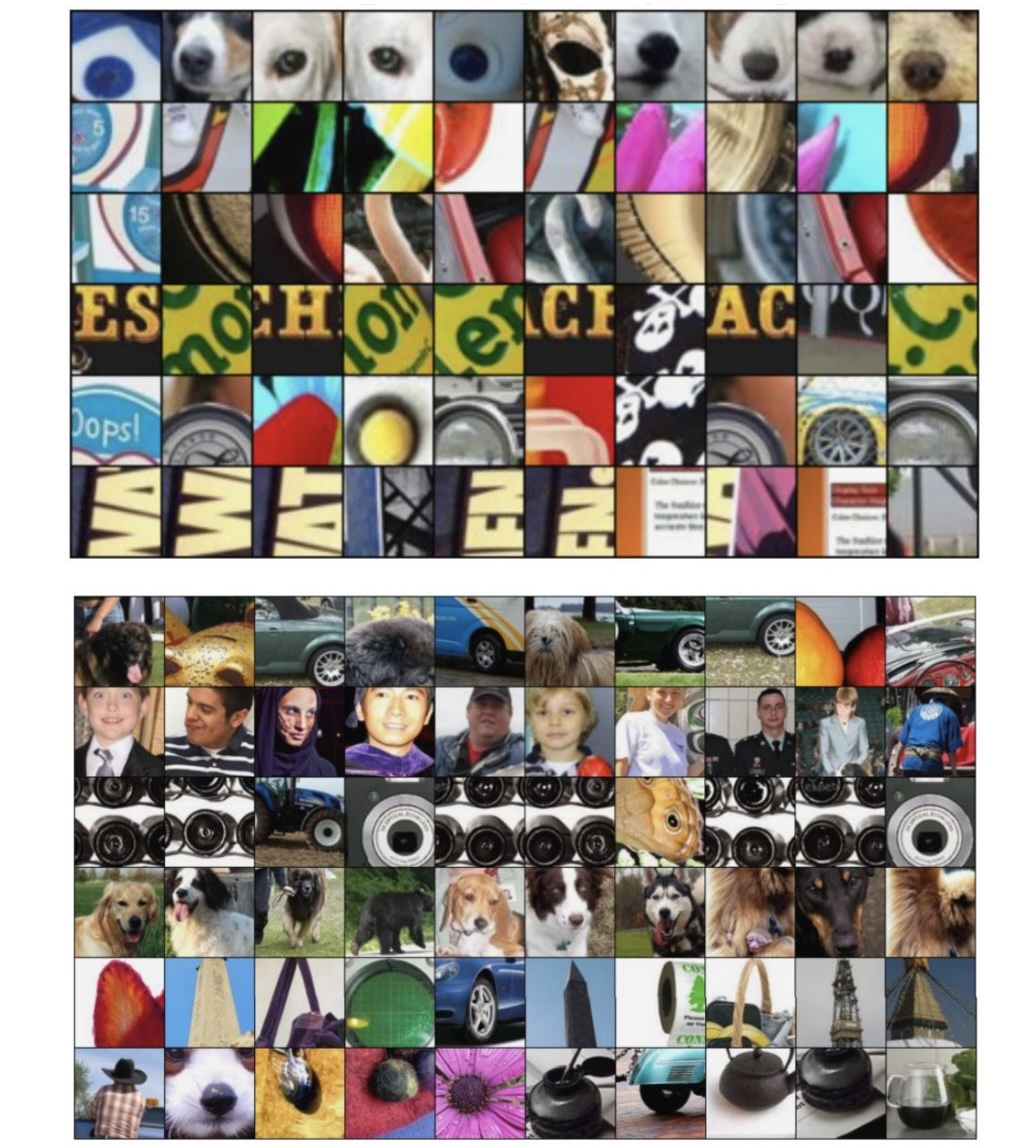
\includegraphics[width=0.5\linewidth]{figs/chapter7/map.jpg}
\end{figure}

\subsection{Occlusion Experiments}

遮盖住输入图像的一部分之后再输入进 CNN，记录分类结果的概率。可以据此做出遮盖不同位置导致不同概率的热点图，如下：

\begin{figure}[H]
    \centering
    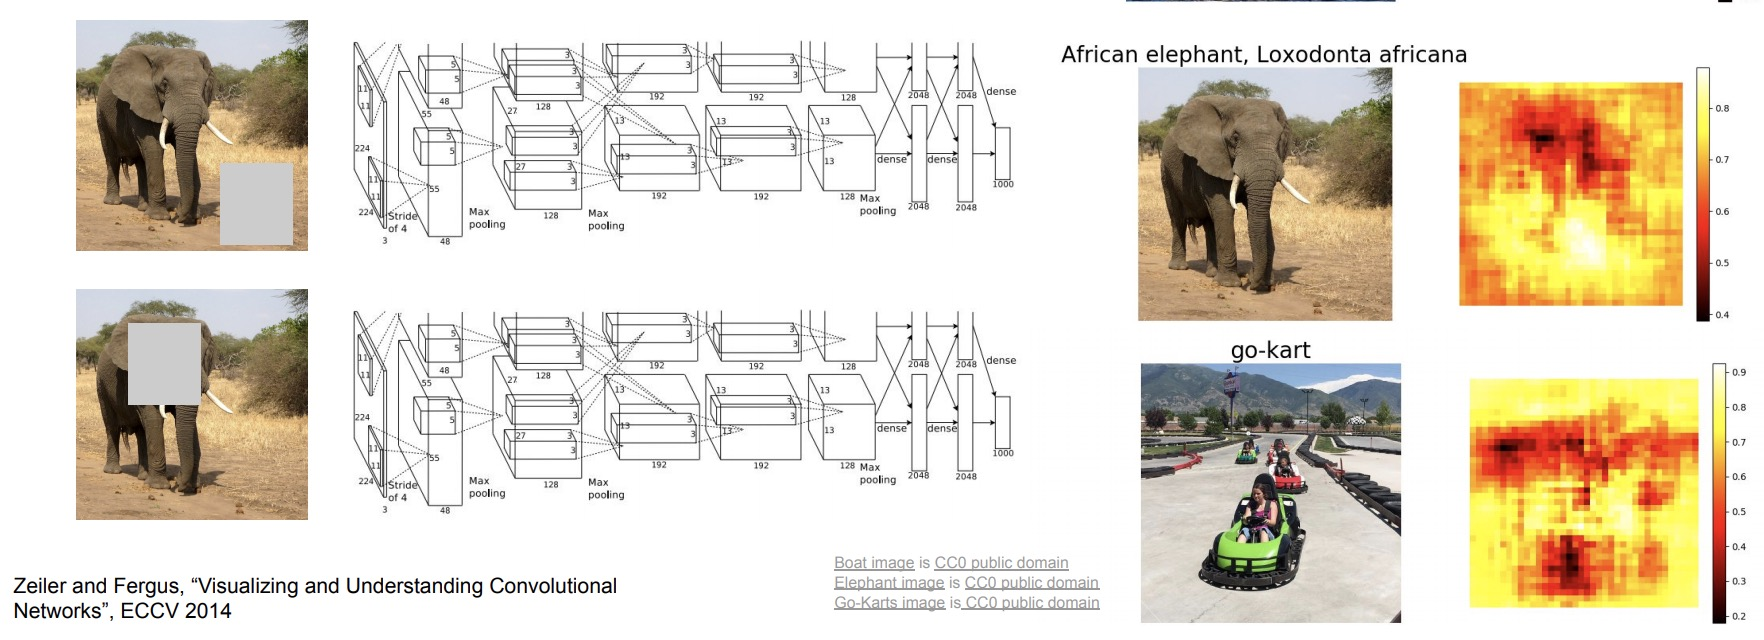
\includegraphics[width=1\linewidth]{figs/chapter7/occlusion.jpg}
\end{figure}

显然，那些导致分类概率急剧变小的像素就是图像里关键的地方。

\subsection{Saliency Maps}

Saliency Maps 和 Occlusion 的目的一样，都是想知道哪些像素对分类结果很重要。

计算每一类的得分对图像像素的梯度，取绝对值并取 RGB 三个 channel 中的最大值。这样做让我们知道如果一个像素发生了微小扰动，相应类的分类得分将发生多大的变化。如果变化很大，自然这个像素对该分类非常重要。

\begin{figure}[H]
    \centering
    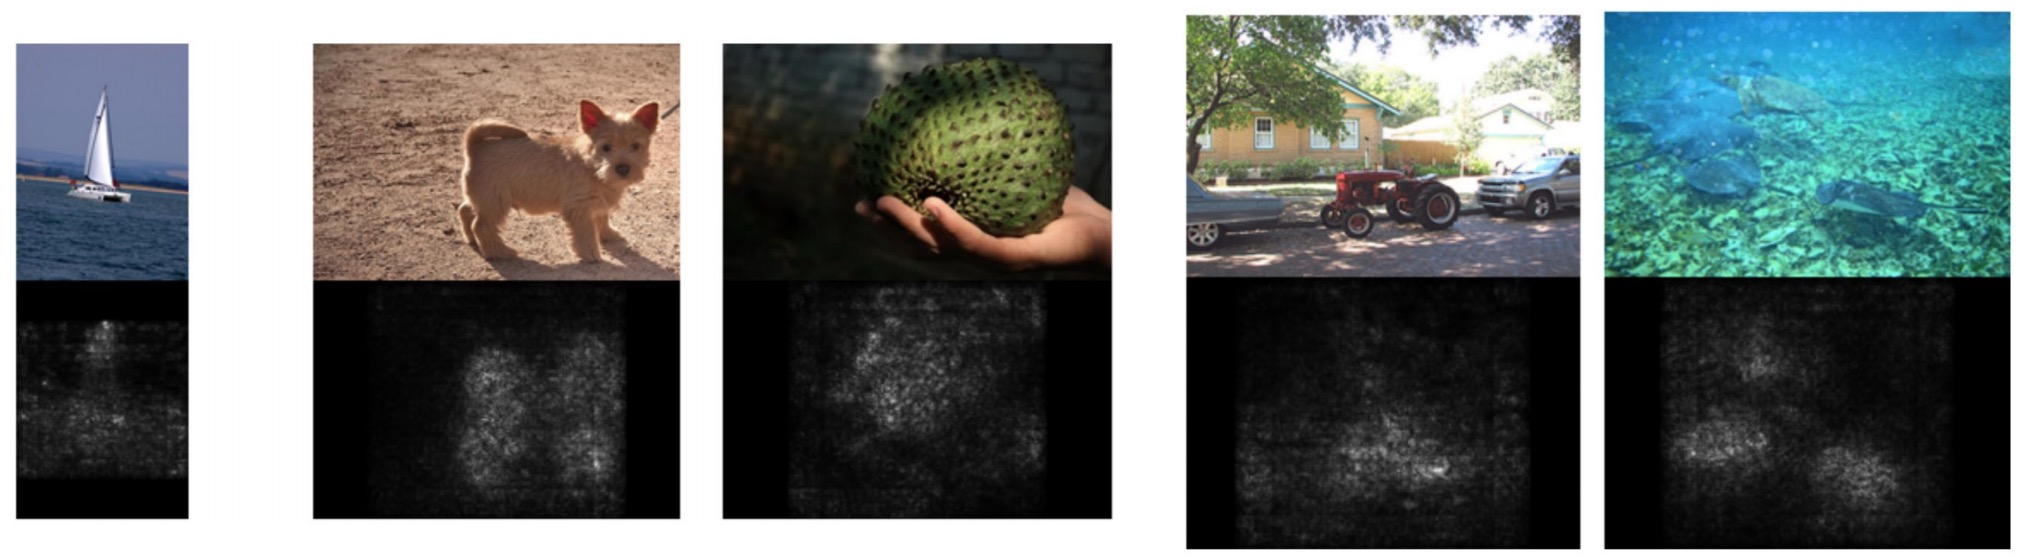
\includegraphics[width=0.8\linewidth]{figs/chapter7/saliency.jpg}
\end{figure}

由此，我们可以想到把 saliency maps 用在 semantic segmentation 中，并且这样做不需要 semantic segmentation 的训练数据。使用 \textbf{GrabCut} 算法可以做到这一点：

\begin{figure}[H]
    \centering
    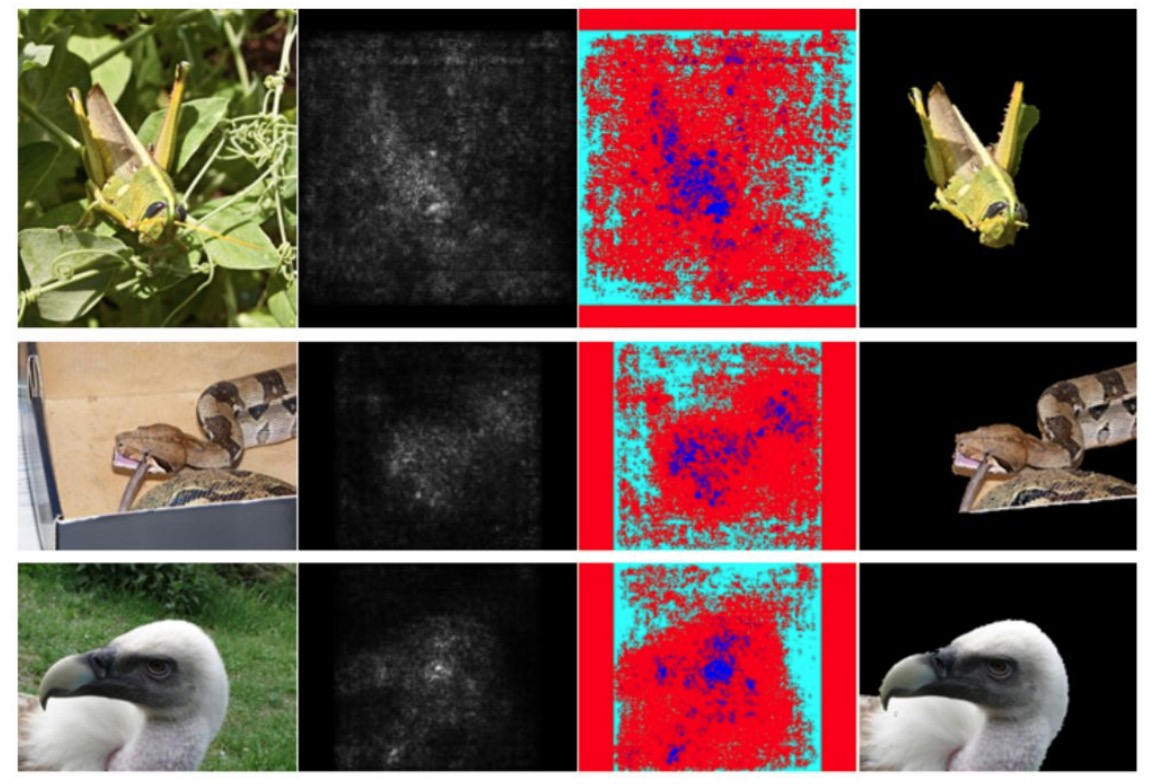
\includegraphics[width=0.8\linewidth]{figs/chapter7/grabcut.jpg}
\end{figure}

\subsection{Intermediate features via (guided) backprop}

借助和 Saliency Maps 类似的想法，如果我们取出神经网络中的某一个神经元并计算其对输入图像各个像素的梯度，那我们也能知道哪些像素对这个神经元非常重要。然而，与通常的 back propagation 不同，我们这时使用 guided backprop，只对通过 ReLU 的正的梯度进行反向传播，这样得到的图像更加清晰。

\begin{figure}[H]
    \centering
    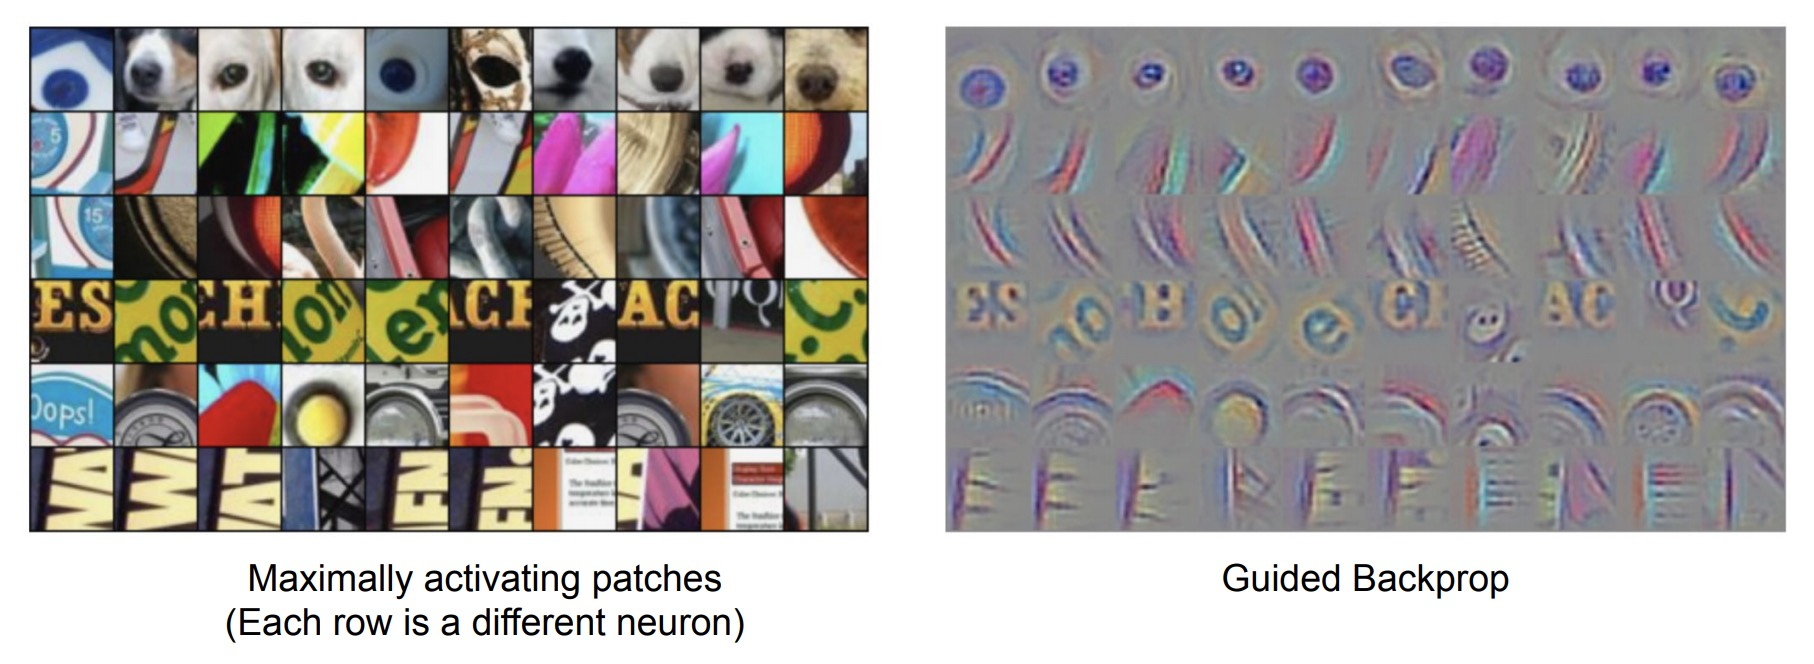
\includegraphics[width=0.8\linewidth]{figs/chapter7/gb.jpg}
\end{figure}

\begin{figure}[H]
    \centering
    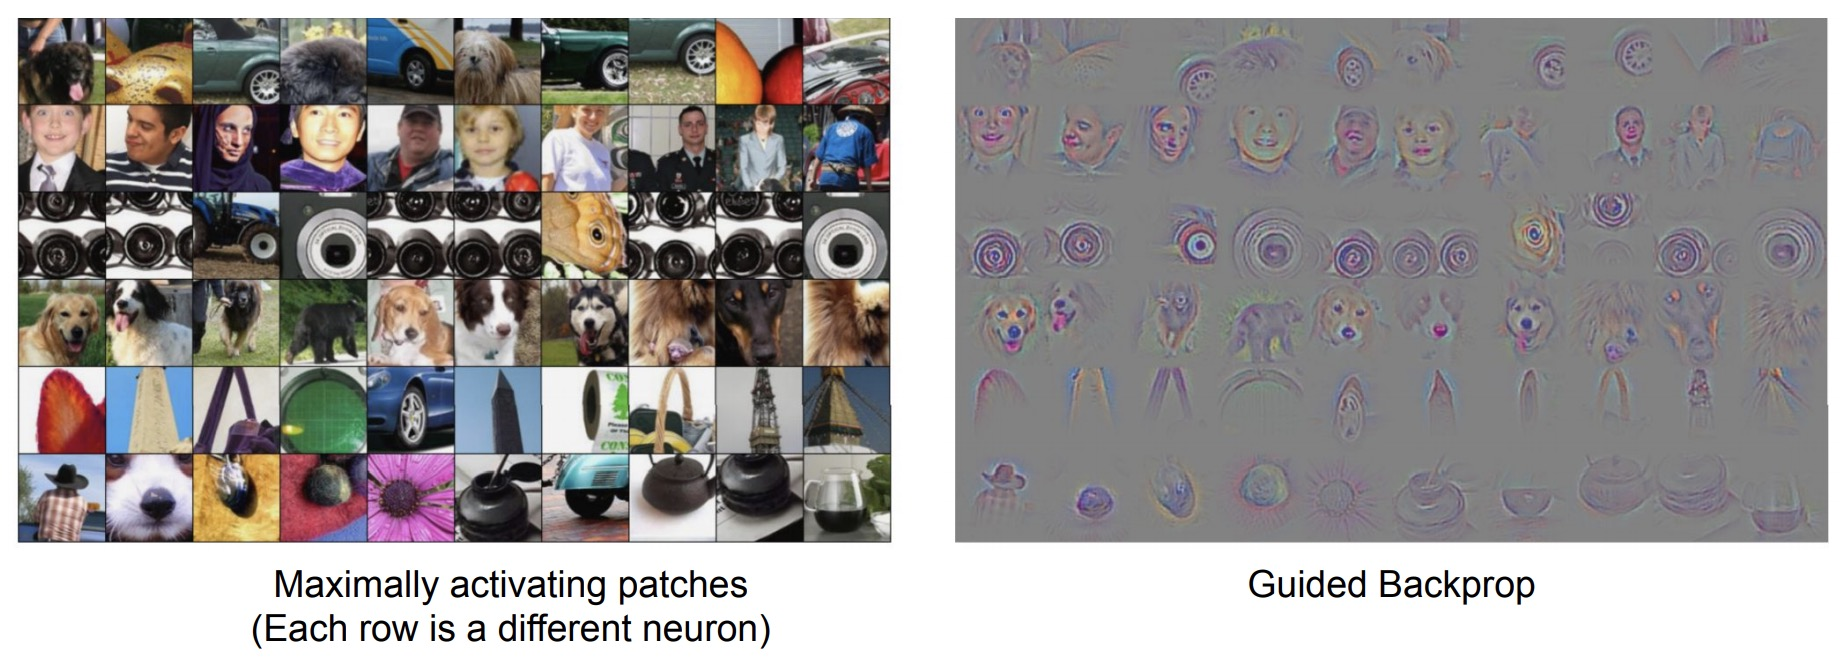
\includegraphics[width=0.8\linewidth]{figs/chapter7/gb2.jpg}
\end{figure}

\subsection{Gradient Ascent}

对于神经网络中的一个神经元，我们想知道什么类型的输入能够激活这个神经元。注意现在和之前的区别在于，我们现在不依赖于输入的数据，而是生成一个使得神经元激活的输入类型。为解决这个问题，我们可以采取 Gradient Ascent.

在 Gradient Descent 中，我们改变参数的值来最小化结果；而 Gradient Ascent 是一个相反的过程，我们固定参数而去改变输入图像的像素，以使得神经元被最大激活或者某一类的得分最大。同时我们需要正则化项，以避免我们生成的图像对我们的网络结构过拟合：
\[
I^*=\arg\max_If(I)+R(I)
\]
其中 $f(I)$ 表示神经元的值或者某一类的得分，而 $R(I)$ 是正则化项。

\subsection{Fooling Images / Adversarial Examples}

首先任选一个输入图像、任选一类，然后更改图像来使得选定类别的分值最大，反复此操作直到网络被 fool.
结果我们发现，一个被更改为错误分类的图像其实并没有肉眼可见的变化。

\begin{figure}[H]
    \centering
    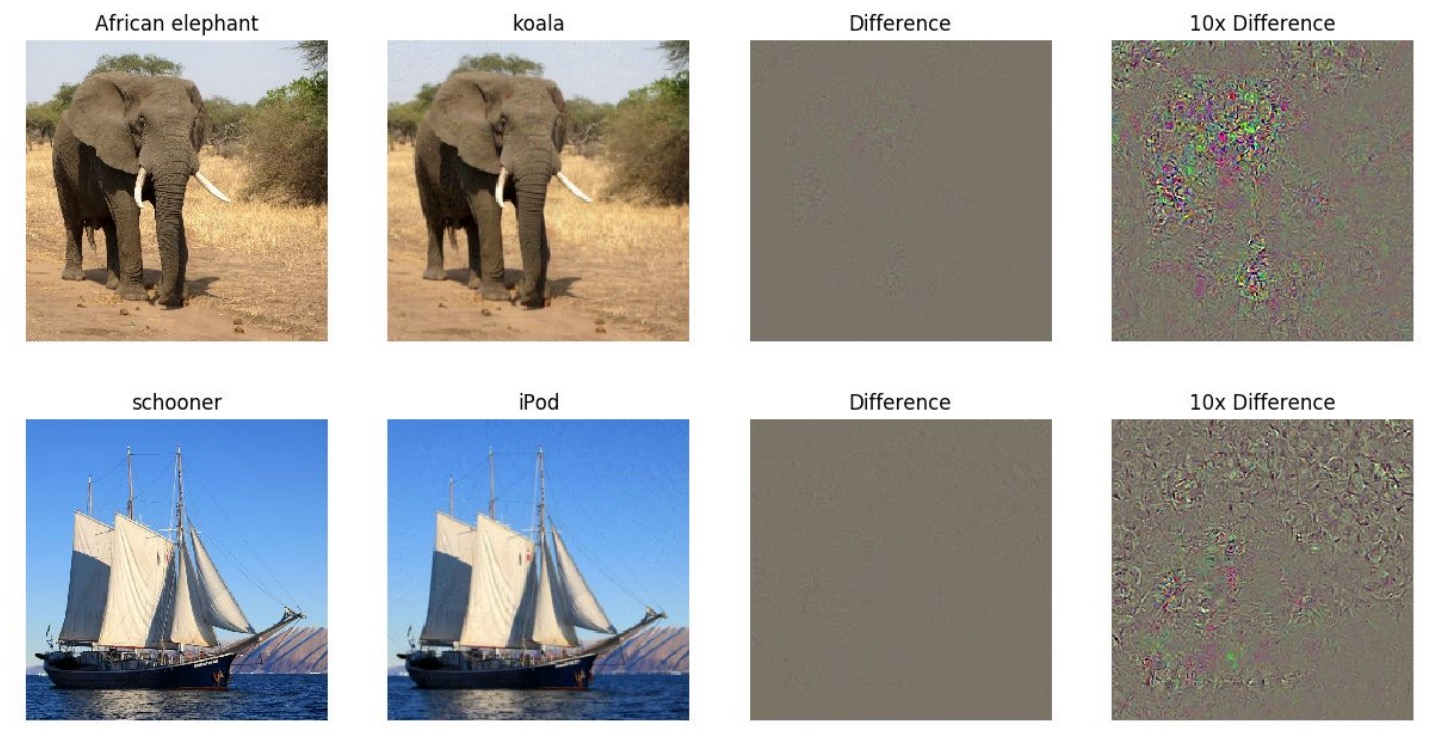
\includegraphics[width=0.8\linewidth]{figs/chapter7/fool.jpg}
\end{figure}

\subsection{DeepDream: Amplify existing features}

对于给定一张图像和选定 CNN 中的某层，反复执行：

\begin{enumerate}
    \item 前向传播到选定的层；
    \item 设置该层的梯度等于其激活值；
    \item 反向传播，计算对输入图像的梯度；
    \item 更新图像
\end{enumerate}
这样做以使得图像的特征被增强。
